\documentclass{article}
\usepackage[utf8]{inputenc}
\usepackage[T2A]{fontenc}
\usepackage[russian]{babel}
\usepackage{graphicx} % Required for inserting images
\usepackage{amsmath}
\usepackage{url}
\usepackage{geometry}
\geometry{a4paper, margin=2cm}

\title{Прогнозирование расщепления \\белков на пептиды.}
\author{Шабаров Игорь}
\date{Декабрь 2025}

\begin{document}

\maketitle

\section{Введение}
\textbf{Белки} — это состоящие из аминокислотных остатков биополимеры, они выполняют ключевые структурные, каталитические и регуляторные функции в клетках. Их функциональная активность определяется не только аминокислотной последовательностью, но и пространственной организацией, стабильностью и временем жизни в клетке.

Неправильно свернутые, повреждённые, короткоживущие регуляторные белки, а также чужеродные белки, попадающие в организм, подвергаются \textbf{протеолизу} — ферментативному расщеплению белковых цепей специализированными протеазами. В ходе протеолиза образуются \textbf{пептиды} — относительно короткие фрагменты белков, как правило длиной до нескольких десятков аминокислотных остатков. Эти пептиды могут обладать самостоятельной биологической активностью, участвовать в сигнальных каскадах, иммунных процессах и регуляции клеточной активности.

Понимание механизмов протеолиза и состава образующихся пептидов имеет особое значение в контексте разработки лекарственных препаратов и вакцин, многие из них несут в себе чужеродные белки, которые расщепляются пептиды, распознаваемые иммунной системой. Таким образом, предсказание продуктов протеолиза позволяет более точно моделировать иммунный ответ и повышать эффективность биомедицинских разработок.

\subsection{Задача предсказания протеолиза и её значимость}
Поскольку в геномных и протеомных данных, как правило, представлена аминокислотная последовательность белка-предшественника, а не конечные продукты его расщепления, задача предсказания результатов протеолиза и границ образующихся пептидов является принципиально важной. Корректное предсказание этих процессов позволяет реконструировать набор потенциально образующихся пептидов и тем самым уточнять функциональную интерпретацию протеомных данных.

\subsection{Области применения}
\begin{itemize}
  \item \textbf{Протеомика и реконструкция протеолитических путей.}\\
  Модели предсказания протеолиза способствуют интерпретации данных масс-спектрометрии, сопоставляя наблюдаемые пептиды с белками-предшественниками, локализуя предполагаемые участки разреза и оценивая влияние вариаций последовательности на паттерны расщепления. 

  \item \textbf{Разработка терапевтических пептидов и вакцин.}\\
  На этапе дизайна позволяют быстро оценить «обрабатываемость» конструкций: какие фрагменты вероятно формируются \textit{in vivo}, а какие паттерны протеолиза могут приводить к нежелательным продуктам или ускоренной деградации. Это снижает риск неудачных кандидатов и повышает эффективность селекции препаратов.

  \item \textbf{Инженерия и дизайн белков.}\\
  Предсказание протеолиза используется для предотвращения нежелательного расщепления, целенаправленного использования управляющих паттернов и проектирования предшественников, формирующих заданный набор пептидов в клеточных условиях. Тем самым модели выступают как автоматизированный фильтр качества при проектировании последовательностей.

  \item \textbf{Патологии протеолиза.}\\
  В ряде патологий (нейродегенеративных, онкологических, эндокринных) нарушается процесс протеолиза, появляются нежелательные паттерны разреза. Модели предсказания деградации белков помогают в их обнаружении и сопоставлении ожидаемых и наблюдаемых паттернов между контрольными и патологическими образцами, что позволяет формировать гипотезы о механизмах накопления токсичных фрагментов.
\end{itemize}

\section{Постановка задачи}

Рассматривается белок-предшественник, заданный аминокислотной последовательностью
$$
x = (a_1, a_2, \dots, a_L), \quad a_t \in \Omega,
$$
где $\Omega$ --- конечный алфавит аминокислотных остатков, используемый в датасете, а $L$ --- длина последовательности.

Целью является предсказать, какие непрерывные фрагменты этой последовательности
образуют зрелые пептиды (и, при необходимости, пропептиды). Формально,
задача может быть записана как структурированная разметка
последовательности: каждой позиции $t$ ставится в соответствие метка
$$
  y_t \in \mathcal{Y}, \quad \mathcal{Y} = \{\text{None}, \text{Peptide}, \text{Propeptide}\},
$$
Модель должна аппроксимировать неизвестное распределение $p(y \mid x)$ и находить
наиболее вероятную разметку $\hat{y}$ (а значит, и сегментацию $\hat{S}$) для данной
аминокислотной последовательности.

Интуитивно, задача состоит в том, чтобы по буквенной последовательности аминокислот
выделить участки, которые с наибольшей вероятностью будут образовывать пептиды после
расщепления предшественника. Например:
$$
  MGKRALRRSGKVRNL \rightarrow MGK | RALR | RSGK | VR | NL
$$

\section{Обзор существующих решений}

Для задач предсказания расщепления пептидов можно выделить два ключевых класса методов: специализированные модели предсказания протеолитических пептидов и общие protein language models (pLM), используемые как источники эмбеддингов.

\subsection{Специализированные модели предсказания протеолитических пептидов}

На данный момент одной из немногих явно нацеленных на задачу предсказания протеолитических пептидов  является модель \textbf{DeepPeptide}~\cite{deeppeptide2023}. Она использует аннотации типов \texttt{PEPTIDE} и \texttt{PROPEP} из датасетов \textbf{UniProtKB/Swiss-Prot}~\cite{uniprot2025} и формулирует задачу как сегментацию белка-предшественника на пептиды и пропептиды. Архитектура включает:
\begin{itemize}
    \item эмбеддинги из protein LM семейства ESM-2~\cite{ESM-family};
    \item стек CNN--BiLSTM--CNN поверх per-residue эмбеддингов;
    \item линейно-цепной CRF с расширенным пространством состояний, который формирует целостные сегменты с ограничениями по длине.
\end{itemize}
Такой декодер позволяет оптимизировать качество именно на уровне целых пептидов, а не отдельных позиций.

\subsection{Protein language models как источник эмбеддингов}

Большинство современных подходов для предсказания  протеолитических пептидов  (включая возможные модификации DeepPeptide) опираются на pLM как на энкодеры последовательности:

\begin{itemize}
    \item \textbf{ESM-2}~\cite{ESM-family}: encoder-only трансформер BERT-типа, обученный задачей masked language modeling на UniRef; даёт контекстные per-residue эмбеддинги, которые в DeepPeptide используются как входные признаки.
    \item \textbf{ESM Cambrian (ESM C)}~\cite{esm_cambrian_blog_2024}: более новое семейство encoder-only трансформеров с RoPE и SwiGLU, оптимизированное по качеству/ресурсам; рассматривается как drop-in замена ESM-2 для многих задач, включая предсказание протеолиза.
    \item \textbf{Ankh}~\cite{ankh2023}: небольшая encoder--decoder модель, в которой на практике используют только энкодер для получения per-residue эмбеддингов; даёт сопоставимое или лучшее качество, чем ProtT5/ESM-2, при меньшем размере.
\end{itemize}

В рамках данной задачи pLM используются как frozen-энкодеры: аминокислотная последовательность переводится в матрицу эмбеддингов $L \times d$, поверх которой обучается специализированная модель сегментации.

\subsection{Генеративные и структурные модели}

Генеративные модели белков, такие как \textbf{ESM3}~\cite{ESM-family} и латентная диффузионная модель \textbf{DiMA}~\cite{dima2024}, ориентированы преимущественно на задачу дизайна новых белков и пептидов. Хотя они не решают задачу предсказания результатов расщепления напрямую, такие модели могут быть использованы на этапе генерации или предварительного отбора кандидатных последовательностей, которые затем анализируются специализированными моделями протеолиза.

Структурные модели, в частности \textbf{AlphaFold~3}~\cite{alphafold3_2024}, восстанавливают трёхмерную структуру белков, пептидов и их комплексов и тем самым предоставляют пространственный контекст, недоступный при анализе одной лишь аминокислотной последовательности. Получаемые при этом внутренние представления и структурные характеристики могут быть использованы для предсказания протеолиза, например в виде входных представлений для моделей машинного обучения или в качестве дополнительного источника информации при анализе паттернов расщепления. Кроме того, структурные модели могут применяться для последующей валидации предсказанных пептидов и оценки их структурной реализуемости.

\section{План дальнейших действий}

Поскольку одной из немногих моделей с неплохим качеством для задачи предсказания протеолитических пептидов  является \textbf{DeepPeptide}~\cite{deeppeptide2023}, подобная архитектура кажется перспективной, но вероятно она не идеальна. В качестве ближайших экспериментов планируется рассмотреть модификации архитектуры \textbf{DeepPeptide} и проверить, как это отразится на качестве. Возможные модификации:
\begin{itemize}
    \item Замена источника эмбеддингов на более современные модели. (\textbf{ESM C, Ankh, etc.})
    \item Выбор наиболее удачного скрытого слоя моделей генерации эмбеддингов.
    \item Добавление структурных эмбеддингов.
    \item Использовать маленький Transformer-encoder поверх эмбеддингов вместо/вместе с Conv/LSTM.
\end{itemize}
Также кроме изменений архитектуры можно попробовать использовать contrastive learning, чтобы эмбеддинги лучше подходили к нашей задаче. Можно дообучать сами модели-генераторы эмбеддингов, и/или обучать проекционную голову для коррекции эмбеддингов уже после их генерации.

\section{Предварительные результаты проведённых экспериментов}
\centering
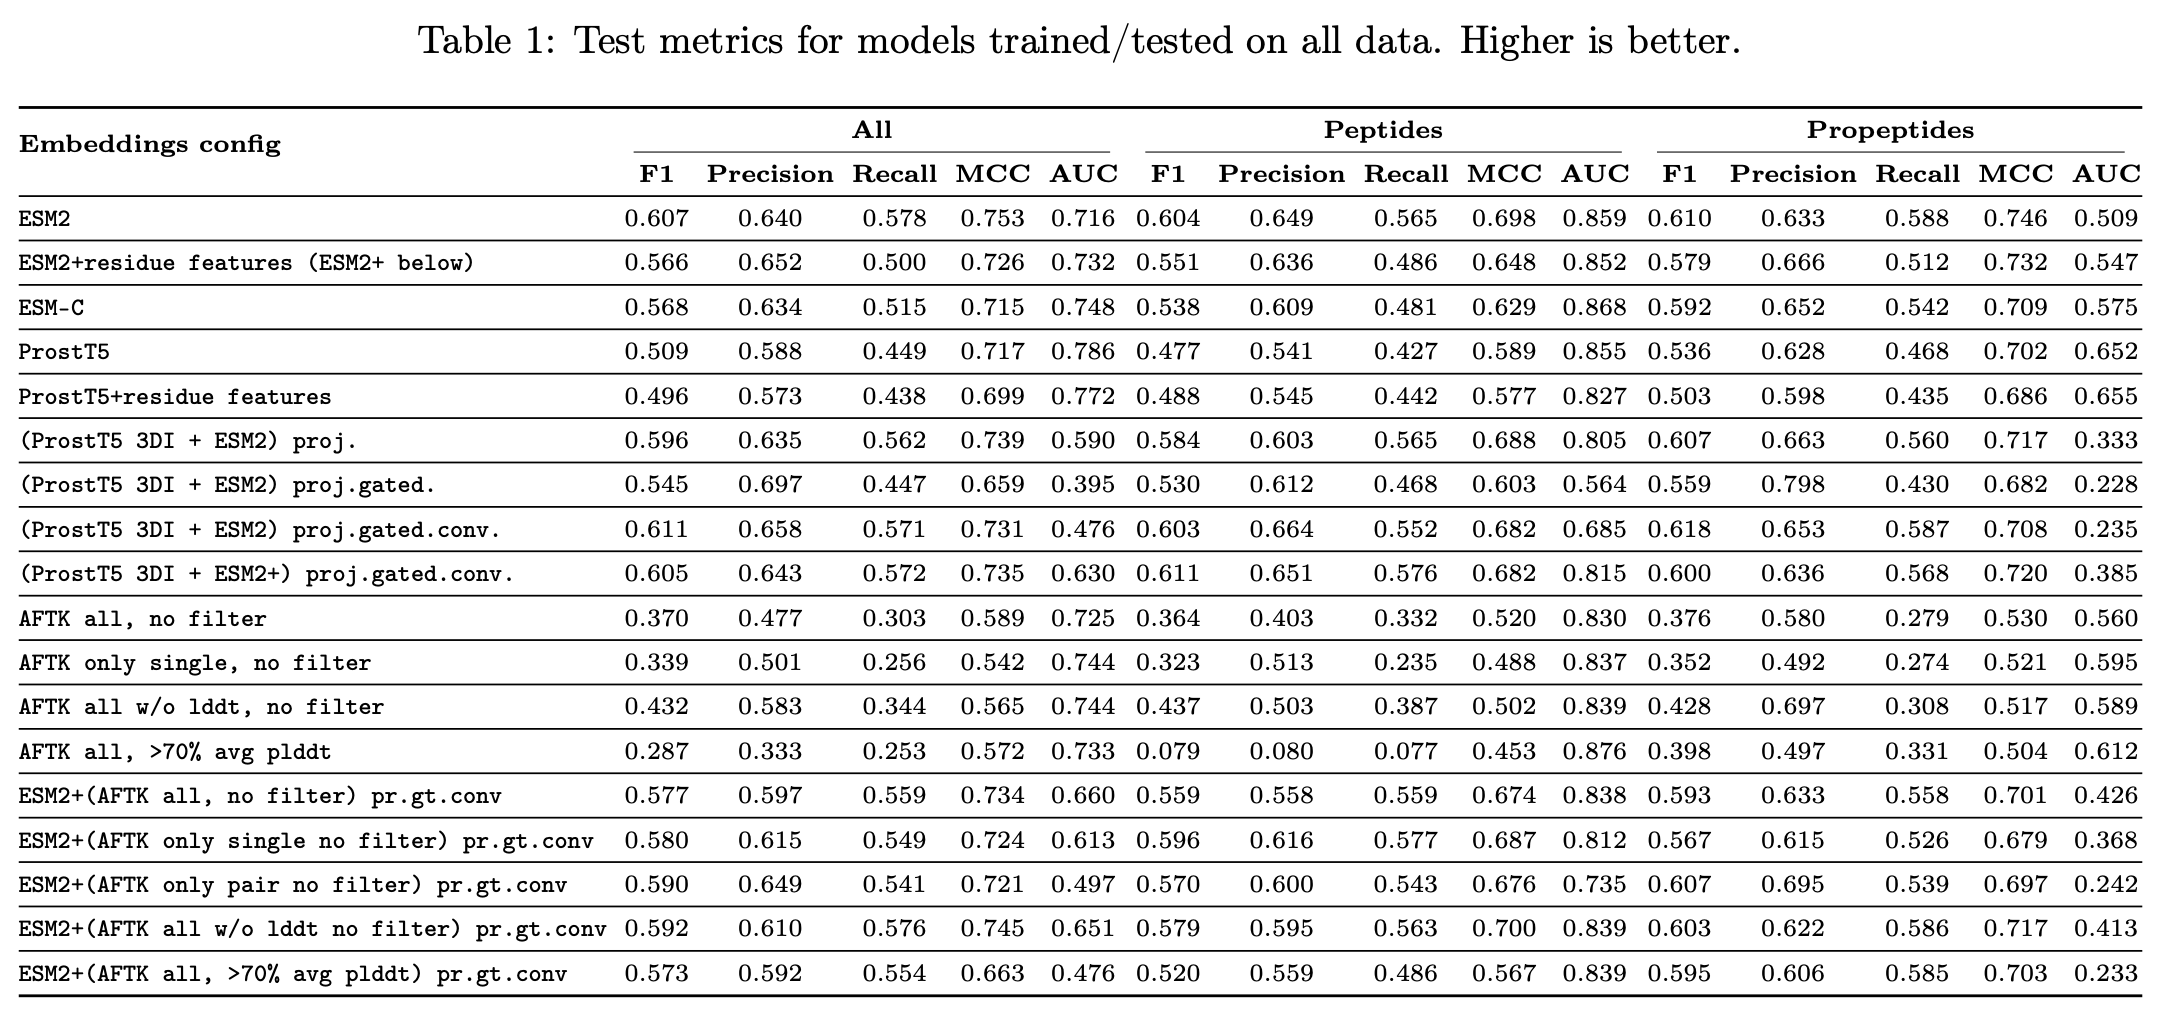
\includegraphics[width=1.0\linewidth]{Experiments.png}

\bibliographystyle{plain}
\bibliography{refs}

\end{document}